\section{Ejercicio 2}

\subsection{Descripci\'on del problema} \label{ej_2:descripcion}

El problema se trata de un conjunto de ciudades hubicadas a cierta distancia entre ellas, las cuales todas deben de ser provistas de gas.
Para \'esto, tenemos una cantidad $k$ de centrales distribuidoras de gas, y tuber\'ias para conectar ciudades.
Una ciudad tiene gas si hay un camino de tuber\'ias que llegue hasta una central distribuidora, es decir,
si una ciudad est\'a conectada a otra ciudad por una tuber\'ia y a su vez \'esta est\'a conectada a otra ciudad
por medio de una tuber\'ia la cual tiene una central distribuidora, entonces las 3 ciudades tienen gas.
Se pide lograr que todas las ciudades tengan gas, pero que la longitud de la tuber\'ia m\'as larga de la soluci\'on
debe ser la m\'as corta posible. La longitud de una tuber\'ia es igual a la distancia entre las 2 ciudades.

El algoritmo tiene que tener una complejidad de $O(n^2)$, con $n$ la cantidad de ciudades.

De a partir de ahora, $k$ va a ser siempre la cantidad de centrales distribuidoras disponibles, y $n$ la cantidad de ciudades.

\subsubsection{Ejemplo}

Como entrada podemos tener 6 ciudades y 2 centrales distribuidoras, como en la Figura \ref{ej_2:ej:entrada}, y la soluci\'on que se busca es como indica la Figura \ref{ej_2:ej:solucion}.

\begin{figure}[htbp]
\centering
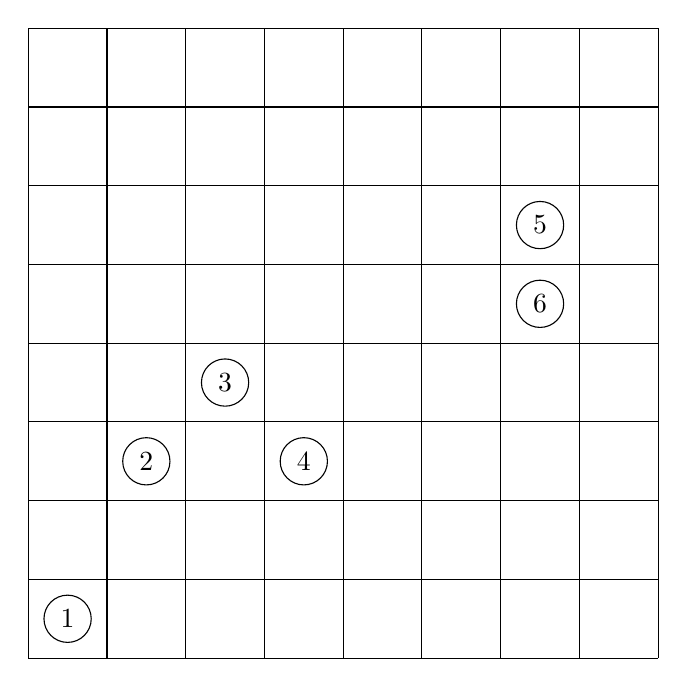
\begin{tikzpicture}

	\draw[xshift=0.5cm, yshift=0.5cm] (-1,-1) grid (7,7);
	\draw (0,0) circle [radius=0.3];
	\draw (0,0) node {1};
	\draw (1,2) circle [radius=0.3];
	\draw (1,2) node {2};
	\draw (2,3) circle [radius=0.3];
	\draw (2,3) node {3};
	\draw (3,2) circle [radius=0.3];
	\draw (3,2) node {4};
	\draw (6,5) circle [radius=0.3];
	\draw (6,5) node {5};
	\draw (6,4) circle [radius=0.3];
	\draw (6,4) node {6};
\end{tikzpicture}

\emph{Se tienen 2 centrales disponibles}

\caption{La entrada del problema, con las 5 ciudades y la cantidad de centrales}
\label{ej_2:ej:entrada}
\end{figure}

\begin{figure}[htbp]
\centering
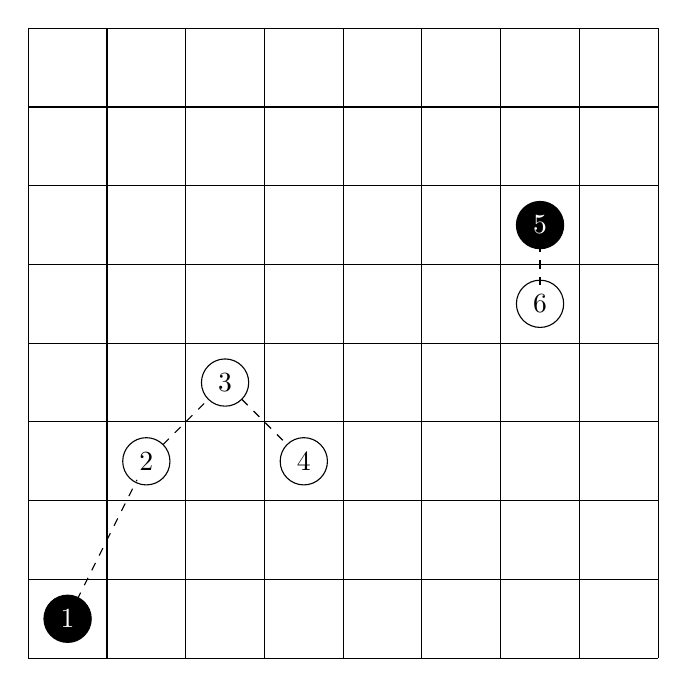
\begin{tikzpicture}
	\draw[xshift=0.5cm, yshift=0.5cm] (-1,-1) grid (7,7);
	\draw[fill=black] (0,0) circle [radius=0.3];
	\draw[white] node (v1) at (0,0) {1};
	\draw (1,2) circle [radius=0.3];
	\draw node (v2) at (1,2) {2};
	\draw[style=dashed] (v1) -- (v2);
	\draw (2,3) circle [radius=0.3];
	\draw node (v3) at (2,3) {3};
	\draw[style=dashed] (v2) -- (v3);
	\draw (3,2) circle [radius=0.3];
	\draw node (v4) at (3,2) {4};
	\draw[style=dashed] (v3) -- (v4);
	\draw[fill=black] (6,5) circle [radius=0.3];
	\draw[white] node (v5) at (6,5) {5};
	\draw (6,4) circle [radius=0.3];
	\draw node (v6) at (6,4) {6};
	\draw[style=dashed] (v5) -- (v6);
\end{tikzpicture}
\caption{La soluci\'on al problema de la Figura \ref{ej_2:ej:entrada}, los nodos negros son los que contienen las centrales de distribuci\'on}
\label{ej_2:ej:solucion}
\end{figure}


\subsection{Ideas para la resoluci\'on} \label{ej_2:idea}

Para la resoluci\'on del problema, se puede penzar en un \emph{grafo}, donde las ciudades son nodos y las tuber\'ias las aristas,
cada arista va a tener una distancia asociada que es la distancia entre los nodos (ciudades) que conecta.

Como cada ciudad tiene gas si hay un camino hasta una central distribuidora, entonces todas las ciudades que se conectan
a una misma central pertenecen a una misma componente conexa. Como tenemos un m\'aximo de $k$ centrales, la soluci\'on tiene que tener un m\'aximo de $k$ componentes conexas y las centrales se colocar\'an cada una en una componente conexa y en cualquier ciudad dentro de la componente conexa, ya que la distancia de las aristas dentro de una componente conexa no se ver\'a modificada si se cambia de nodo la central dentro de la misma componente conexa.

Entonces, la soluci\'on que se pide es que el grafo tenga a lo sumo $k$ componentes conexas, y que la distancia de la arista mas larga, sea la m\'as corta posible.

Una idea que se propone es comenzar con todos los nodos sueltos, sin ninguna arista conectada,
y calcular todas las distancias entre todos los nodos, es decir, calcular todas las tuber\'ias posibles con sus respectivas distancias.
Luego se ordenar\'an las aristas (tuber\'ias) de menor a mayor de acuerdo a sus longitudes.
Se calcula si la cantidad de componentes conexas es menor o igual a $k$, si es as\'i, entonces el algoritmo termina, sino coloca la tuber\'ia m\'as corta que no genere un ciclo y contin\'ua preguntando sobre la cantidad de componentes conexas e iterando sobre las aristas siguiendo el orden de menor a mayor.
Es parecido al algoritmo de \emph{Kruskal}.

Para mejorar la complejidad del algoritmo, en vez de calcular la distancia de todos las aristas e iterar sobre todas las aristas, requiriendo ordenar por peso \emph{todas} las aristas, primero creamos un \'arbol generador m\'inimo (con las aristas m\'as cortas posibles), con una idea como el algoritmo de Prim y que tenga de cota $O(n^2)$,
qued\'andonos $n - 1$ aristas, y luego, al igual que antes, se ordenan y se recorren esas $n - 1$ aristas de menor a mayor.

En la secci\'on \ref{ej_2:algoritmo} se propone un pseudoc\'odigo, en la secci\'on \ref{ej_2:ejemplo} se ver\'a un ejemplo de ejecuci\'on del algoritmo,
en la secci\'on \ref{ej_2:justificacion} se justificar\'a la correctitud, y en la secci\'on \ref{ej_2:cota} se har\'a el c\'alculo de la complejidad del algoritmo.

\subsubsection{Algoritmo} \label{ej_2:algoritmo}

\begin{algorithm}[!h]
\caption{minimizarTuberias} \label{ej_2:pseudo}
\end{algorithm}
\begin{algorithmic}[1]
	\Require \emph{centrales}: cantidad de centrales disponibles, mayor que 0
	\Require \emph{ciudades}: las ciudades con sus posiciones
	\Require \emph{n}: cantidad de ciudades en el par\'ametro \emph{ciudades}
	\Statex
	\Ensure Retorna el grafo tal que hay tanas componentes conexas como \emph{centrales}, y que la arista m\'as larga es la m\'as corta posible
	\Statex
	\Procedure{minimizarTuberias}{Entero: centrales, Array: ciudades, Entero: n}{$\to$ Grafo}
		\State Grafo g $\gets$ \Call{NuevoGrafo}{$n$} \Comment{Creo un grafo con $n$ nodos, sin aristas}
		\State $<$bool agregado, entero distancia, entero nodo$>$  nodos[n] \Comment{La distancia es desde $n$ (\'indice del array) hasta nodos[$n$].nodo}
		\State $<$nodo1, nodo2, distancia$>$ aristas[n - 1]
		\Statex
		\State nodos[0] $\gets$ $<$true, 0, 0$>$ \label{ej_2:pseudo:inicializa}
		\For{i $\gets$ 1; i $<$ n; i$++$} \label{ej_2:pseudo:distancia}
			\State nodos[i] $\gets$ $<$false, \Call{Distancia}{ciudades[i], ciudades[0]}, 0$>$
		\EndFor \label{ej_2:pseudo:fin_inicializa}
		\Statex
		\For{agregados $\gets$ 0; agregados $<$ n - 1; agregados$++$} \label{ej_2:pseudo:crea_arbol}
			\State distancia\_minima $\gets$ $\infty$
			\State nodo\_minimo $\gets$ 0
			\For{i $\gets$ 0; i $<$ n; i$++$} \Comment{Busco el nodo mas cercano al \'arbol que ya tenemos} \label{ej_2:pseudo:mas_cerca}
				\If{nodos[i].agregado = false}
					\If{nodos[i].distancia $<$ distancia\_minima}
						\State distancia\_minima $\gets$ nodos[i].distancia
						\State nodo\_minimo $\gets$ i
					\EndIf
				\EndIf
			\EndFor \label{ej_2:pseudo:fin_mas_cerca}
			\Statex
			\State nodos[nodo\_minimo].agregado $\gets$ true \label{ej_2:pseudo:nodo}
			\State aristas[agregados] $\gets$ $<$nodo\_minimo, nodo[nodo\_minimo].nodo, distancia\_minima$>$ \Comment{Agrego el nodo encontrado} \label{ej_2:pseudo:arista}
			\Statex
			\For{i $\gets$ 0; i $<$ n; i$++$} \Comment{Actualizo la distancia de los nodos no agregados a\'un} \label{ej_2:pseudo:actualiza}
				\If{nodos[i].agregado = false}
					\If{nodos[i].distancia $>$ \Call{Distancia}{ciudades[i], ciudades[nodo\_minimo]}}
						\State nodo[i].distancia $\gets$ \Call{Distancia}{ciudades[i], ciudades[nodo\_minimo}
						\State nodo[i].nodo $\gets$ nodo\_minimo
					\EndIf
				\EndIf
			\EndFor \label{ej_2:pseudo:fin_actualiza}
		\EndFor \label{ej_2:pseudo:fin_crea_arbol}
		\Statex
		\State \Call{Ordenar}{aristas} \Comment{Ordeno las aristas por la distancia} \label{ej_2:pseudo:sort}
		\Statex
		\For{componentes $\gets$ n; componentes $>$ centrales; componentes$--$} \label{ej_2:pseudo:componentes}
			\State \Call{AgregarArista}{g, aristas[n - componentes].nodo1, aristas[n - componentes].nodo2}
		\EndFor \label{ej_2:pseudo:fin_componentes}
		\State retornar $\gets$ g
	\EndProcedure
\end{algorithmic}



\subsubsection{Ejemplo de ejecuci\'on} \label{ej_2:ejemplo}

\subsection{Justificaci\'on del procedimiento} \label{ej_2:justificacion}


%El Algoritmo \ref{ej_2:pseudo} se puede dividir en 4 partes. Primero de la l\'inea \ref{ej_2:pseudo:inicializa} a \ref{ej_2:pseudo:fin_inicializa} inicializa variables,
%luego de la l\'inea \ref{ej_2:pseudo:crea_arbol} a \ref{ej_2:pseudo:fin_crea_arbol} crea un \'arbol generador que la arista de mayor peso sea la menor posible,
%en la l\'inea \ref{ej_2:pseudo:sort} se ordenan las aristas del \'arbol del paso anterior,
%y entre \ref{ej_2:pseudo:componentes} y \ref{ej_2:pseudo:fin_componentes} se busca encontrar la soluci\'on con la arista m\'as corta posible.
%
%C\'omo se explic\'o en la Secci\'on \ref{ej_2:idea}, la idea del algoritmo es buscar el \'arbol con un algoritmo como Prim y luego agregar de a una las aristas de dicho \'arbol en orden de menor peso hasta encontrar la soluci\'on al problema.
%
%Vamos a demostrar que el algoritmo genera un \'arbol generador que minimiza el peso de las aristas (Secci\'on \ref{ej_2:demo:arbol}, y que a partir de las aristas del \'arbol se genera la soluci\'on al problema:
%que haya como m\'axio $k$ componentes conexas y que las aristas sean las m\'as cortas posibles (Secci\'on \ref{ej_2:demo:solucion})
%
%\subsubsection{Obtener el \'arbol} \label{ej_2:demo:arbol}
%
%La entrada que se tiene del problema es una cantidad de ciudades ($n$ nodos), las cuales pueden ser conectadas cualquier ciudad con cualquier ciudad, por lo que la entrada es un grafo completo de $n$ nodos.
%Cada arista tiene un peso, y dicho peso es el que se quiere minimizar, pero el peso de las aristas (la longitud de la tuber\'ia) depende de los nodos que conecta, y no se requiere informaci\'on extra,
%s\'olo con los 2 nodos que conecta la arista se sabe su peso (la distancia entre los nodos)
%
%El Algoritmo \ref{ej_2:pseudo} desde la l\'inea \ref{ej_2:pseudo:inicializa} a \ref{ej_2:pseudo:fin_crea_arbol} obtiene las aristas de longitud m\'inima para obtener el \'arbol generador, colocandolas en el vector \emph{aristas}.
%
%Los pasos del algoritmo son:
%\begin{enumerate}
%	\item Agarra el primer nodo del grafo y lo agrega al \'arbol que va a generar, llamemoslo $T$ (L\'inea \ref{ej_2:pseudo:inicializa})
%	\item Calcula todas las distancias del resto de los nodos hacia el primer nodo (L\'ineas \ref{ej_2:pseudo:distancia} a \ref{ej_2:pseudo:fin_inicializa})
%	\item Recorre la lista de nodos $n - 1$ veces
%	\begin{enumerate}
%		\item Busca el nodo que no pertenezca a $T$ y que tenga la distancia m\'as chica hacia el \'arbol $T$, llamemoslo $v$ (L\'ineas \ref{ej_2:pseudo:mas_cerca} a \ref{ej_2:pseudo:fin_mas_cerca})
%		\item Agrega $v$ al \'arbol $T$ con arista que va desde $v$ hacia el nodo m\'as cercano de $v$ que ya pertenec\'ia a $T$ (L\'ineas \ref{ej_2:pseudo:nodo} y \ref{ej_2:pseudo:arista})
%		\item A los nodos que a\'un no fueron agregados a $T$, le recalcula la distancia hacia el \'arbol $T$ (L\'ineas \ref{ej_2:pseudo:actualiza} a \ref{ej_2:pseudo:fin_actualiza})
%	\end{enumerate}
%\end{enumerate}
%
%\begin{proof}[Demostraci\'on: Los pasos anteriores crean un \'arbol]
%
%El \'arbol que queremos encontrar, $T$, por definici\'on es conexo y tiene $n - 1$ aristas.
%
%El algoritmo divide los nodos en 2 grupos, los agregados a $T$ que son nodos con alguna arista que lo conecta a otro nodo, y los que faltan agregar que son nodos sueltos de grado 0 (llamemoslos $V$) ($T$ y $V$ contienen nodos diferentes), cada vez que agrega una arista, est\'a uniendo un nodo $v \in T$ con un nodo $v' \in V$, sacando $v'$ de $V$ y agreg\'andolo a $T$.
%Como siempre une con una arista con un extremo un nodo que esta en $T$ (que ya est\'a unido a otro nodo en $T$) y en el otro extremo un nodo que est\'a en $V$ y no en $T$ y no es adyacente a ning\'un nodo, entonces $T$ es conexo porque todos los nodos \'estan conectados a $T$ mediante una arista al finalizar la iteraci\'on.
%Como agrega $n - 1$ aristas (L\'inea \ref{ej_2:pseudo:arista}), entonces $T$ es un grafo conexo con $n - 1$ aristas, es decir, un \emph{\'arbol}
%\end{proof}
%
%\begin{proof}[Demostraci\'on: El \'arbol anterior tiene el menor peso]
%En cada paso en que se agrega una nueva arista con un nuevo nodo, el algoritmo busca el nodo m\'as cercano al \'arbol $T$ que se est\'a armando y actualiza las distancias hacia $T$ del resto de los nodos qued\'andose con el m\'inimo entre la distancia vieja a $T$ y la distancia hacia el nuevo nodo que se agreg\'o.
%La distancia a $T$ es el peso de la arista de menor peso que une al nodo con algun nodo de $T$.
%En el algoritmo la distancia de un nodo a $T$ comienza siendo la distancia hacia el \'unico nodo que tiene $T$.
%
%Pruebo que al agregar un nuevo nodo, la distancia a $T$ va a ser la menor entre la vieja distancia a $T$ y la distancia al nuevo nodo que se agreg\'o:
%
%Siendo $d$ la distancia entre un nodo $m$ hacia $T$, significa que hay un nodo $v$ en $T$ tal que:
%\begin{equation}
%	d = distancia(m,T) \equiv
%	(\exists v \in T) (distancia(m,v) = d \land (\forall v' \in T) d <= distancia(m,v')) \label{ej_2:demo:d}
%\end{equation}
%Al agregar un nuevo nodo $w$ a $T$, sucede que las distancias viejas no cambian:
%\begin{equation*}
%	(\forall v' \in (T - w)) d <= distancia(m,v')
%\end{equation*}
%Por lo que al agregar $w$ lo que puede pasar es que $d <= distancia(m,w)$ ( en tal caso sigue valiendo la Equaci\'on \ref{ej_2:demo:d} con $w$ agregado a $T$),
%o puede ser que $d > distancia(m,w)$, entonces en ese caso para que siga valiendo la Equaci\'on \ref{ej_2:demo:d} la distancia hacia $T$ tiene que ser la distancia desde $m$ a $w$.
%Es decir, la distancia a $T$ al agregar un nuevo nodo es la menor entre la distancia vieja y la distancia hacia el nuevo nodo.
%
%El algoritmo en cada paso tiene componentes conexas, por un lado $T$ (el \'arbol que est\'a construyendo) y por otro lado cada uno de los nodos que a\'un no est\'an en $T$.
%Pruebo que teniendo una componente conexa $T$ y varios nodos sueltos, si se agregan los nodos a $T$ en orden de menor distancia entre nodo y $T$, se tiene un \'arbol con las aristas de menor peso posible:
%
%%Sea $T$ el \'arbol ya armado y $T'$ un momento en la iteraci\'on del algoritmo mientras se arma el \'arbol, $T'$ comienza con 1 nodo, y se tiene que agregar aristas para conectarlo con los nodos que a\'un no est\'an en $T'$ para formar $T$,
%%entonces en un instante del armado del \'arbol busco el nodo que tenga la menor distancia a $T'$ (lo llamo $v$) y lo uno mediante la arista $e$ al nodo m\'as cercano dentro de $T'$ (lo llamo $w$).
%%Ahora supongo que existe un mejor \'arbol $A$ tal que llega al mismo paso que $T'$ que $v$ no est\'a en $T'$ y es el m\'as cercano (es decir, $T'$ es subgrafo de $A$ y de $T$) pero no conecto $v$ con $T'$ mediante la arista $e$ (es decir, $v$ con $w$) por lo que $v$ estar\'a conectado a otro nodo en el \'arbol $A$ (porque el \'arbol es conexo) con una arista $e'$ tal que $distancia(e') < distancia(e), e' \in A, e \in T$ haciendo que al finalizar el \'arbol $T$ no minimize la mayor distancia pero $A$ si.
%%Como en $A$, $T'$ no lo conecto con $v$, entonces se tiene que conectar a otro nodo mediante una arista $a, a \in A$. Como el nodo $e$ en $T$ se hab\'ia elegido como el nodo m\'as cercano a $T'$, entonces $a$ no es el m\'as cercano y $distancia(a) > distancia(e)$, por lo que $distancia(e') < distancia(e) < distancia(a)$, como $e \notin A$ y $a \in A$ y $e' \in A$, entonces $A$ tiene una arista ($a$) con mayor distancia que la que tiene $T$, lo que contradice la suposici\'on de que $A$ sea el que minimize la distancia en vez de $T$.
%\end{proof}
%
%\subsubsection{Soluci\'on al problema} \label{ej_2:demo:solucion}
%Teniendo ya un \'arbol $T$ que contiene las aristas m\'as cortas posible, queremos armar $S$ tal que sea la soluci\'on al problema (que contenga $k$ componentes conexas como m\'aximo y que la mayor distancia sea la menor posible).
%
%\begin{proof}
%
%Luego de armar $T$, lo que se hace es ordenar las aristas de $T$ de menor a mayor seg\'un su peso (L\'inea \ref{ej_2:pseudo:sort}) y se agregan de a 1 y en cada paso se est\'a disminuyendo en 1 la cantidad de componentes conexas (porque en el \'arbol no hay ciclos)
%hasta tener $k$ componentes conexas. Como se agregan en orden de menor peso a mayor, las aristas que no se agregaron a $S$ son todas de mayor peso que las que s\'i est\'an en $S$. Suponemos entonces que se quitase la arista de mayor peso de $S$ (llamada $v$) para que
%tener la soluci\'on $S'$ tenga como mayor peso una arista m\'as corta, como $S$ no tiene ciclos (por ser subgrafo del \'arbol $T$) entonces al quitar $v$ se aumentar\'a en 1 la cantidad de componentes conexas, haciendo que sea mayor a $k$, y como no es soluci\'on se necesitar\'a colocar otra arista que no est\'e en $S$ y que no sea $v$ (porque $v$ se sac\'o para mejorar la soluci\'on), y como todas las aristas que no est\'an en $S$ son de mayor peso que las que s\'i, entonces quidando $v$ se tiene que agregar una arista de mayor peso que $v$ a $S$, haciendo que $S'$ tenga la arista m\'as larga, m\'as larga que la que ten\'ia $S$ ($v$) (valga la redundancia), contradiciendo la suposici\'on de agregando las aristas en orden y que quitando la arista m\'as larga de $S$, se obtiene un $S'$ que es mejor soluci\'on.
%\end{proof}

\subsection{Cota de complejidad} \label{ej_2:cota}

Se analiza la complejidad de algoritmo \ref{ej_2:pseudo}, para \'esto se supone que el c\'alculo de la distancia entre ciudades (el peso de las aristas/tuber\'ias) se realiza en $O(1)$

La cantidad de nodos se representar\'a como $n$, y la cantidad de centrales como $k$.

\begin{itemize}
	\item La inicializaci\'on de unas variables se realiza de la l\'inea \ref{ej_2:pseudo:inicializa} a \ref{ej_2:pseudo:fin_inicializa}, y se realizan $n$ iteraciones calculando la distancia y guardando en un vector, quedando $O(n)$
	\item Para la creaci\'on del AGM entre las l\'ineas \ref{ej_2:pseudo:crea_arbol} a \ref{ej_2:pseudo:fin_crea_arbol} realiza $n - 1$ iteraciones
	\begin{itemize}
		\item L\'ineas \ref{ej_2:pseudo:mas_cerca} a \ref{ej_2:pseudo:fin_mas_cerca}, busca el nodo m\'as cercano, realizando $n$ iteraciones de comparaciones y asignaciones que son $O(1)$, quedandonos $O(n)$
		\item Las l\'ineas \ref{ej_2:pseudo:nodo} y \ref{ej_2:pseudo:arista} son $O(1)$
		\item La actualizaci\'on de las distancias, entre las l\'ineas \ref{ej_2:pseudo:actualiza} y \ref{ej_2:pseudo:fin_actualiza} realiza $n$ iteraciones de comparaciones y asignaciones que son $O(1)$, quedandonos $O(n)$
	\end{itemize}
	\item Ordenar las aristas en la l\'inea \ref{ej_2:pseudo:sort}, y se realizan sobre las aristas agregadas en la iteraci\'on anterior, la cual agrega $n-1$ aristas, entonces se ordenan $n - 1$ elementos. Al $n$ no estar acotado, se puede realizar con algoritmos como \emph{MergeSort} o \emph{HeapSort} en $O(n \log n)$
	\item Entre las l\'ineas \ref{ej_2:pseudo:componentes} y \ref{ej_2:pseudo:fin_componentes} se realizan $n - k$ iteraciones, implementando el grafo \emph{g} en una \emph{matriz de adyacencia}, \emph{AgregarArista} se realiza en $O(1)$, quedandonos una complejidad de $O(n - k)$. Notar que si $k > n$, no se realiza ninguna iteraci\'on.
\end{itemize}

Bajo \'este an\'alisis, la complejidad nos queda (\ref{ej_2:cota:formula})

\begin{equation}
\label{ej_2:cota:formula}
\begin{split}
O(n) + (n-1)*(O(n) + O(1) + O(n)) + O(n \log n) + O(n - k) \\
=
O(n) + O(n^2) + O(n) + O(n^2) + O(n \log n) + O(n - k) \\
=
O(2n) + O(2n^2) + O(n \log n) + O(n - k) \\
= O(n^2)
\end{split}
\end{equation}

Cumpliendo as\'i la complejidad requerida.

\subsection{Casos de prueba y resultado del programa} \label{ej_2:casos}

\subsection{Mediciones de performance} \label{ej_2:performance}

\subsection{Concluciones} \label{ej_2:concluciones}

